\section{Scattering Part III}
\subsection{Review of Last Class}
Last time we derived the integral form of the Schrodinger equation:
\begin{equation}\label{eq-Seintegral}
    \psi(r) = \psi_0(r) - \frac{1}{4\pi}\int \frac{e^{ik\abs{\v{r} - \v{r}'}}}{r}\frac{2mV(r')}{\hbar^2}\psi(r')d^3r'
\end{equation}
And by applying the Schrodinger operator to both side, we can confirm that this is indeed the case. Our Green function is:
\begin{equation}
    G(\v{r} - \v{r}') = -\frac{1}{4\pi}\frac{e^{ik\abs{\v{r} - \v{r}'}}}{\v{r} - \v{r}'}
\end{equation}
so writing $U(r') = \frac{2mV(r')}{\hbar^2}$, we have:
\begin{equation}
    \psi(r) = \psi_0(r) + \int \psi(r')G(\v{r} - \v{r}')U(r')d^3r'
\end{equation}
We derived a first-order scattering approximation via Fermi's golden rules, and also through perturbation theory. When we do PT, we consider a solution of the form:
\begin{equation}
    \psi = \psi^{(0)} + \psi^{(1)} + \psi^{(2)} + \ldots
\end{equation}
We say that:
\begin{equation}
    \psi^{(0)} \sim 1, \psi^{(1)} \sim U^1, \psi^{(2)} \sim U^2
\end{equation}
Our $\psi^{(0)}$ is nothing but the incoming wave:
\begin{equation}
    \psi^{(0)}(\v{r}) = e^{i\v{k}_{in}\cdot \v{r}}
\end{equation}
for the Green function, at very large distances we found:
\begin{equation}
    G \to -\frac{e^{ikr}}{4\pi r} e^{-i\v{k}_f \cdot \v{r}}
\end{equation}
We exactly computed the first order of perturbation theory:
\begin{equation}
    \psi^{(1)} = - \frac{e^{ikr}}{4\pi r} \int U(r')e^{-i\v{q} \cdot \v{r}'}d^3r'
\end{equation}
Which is exactly the Fourier transform - the same thing we got from the Fermi's golden rule derivation.

\subsection{Second-Order corrections}
Now we consider $\psi^{(2)}$. To this end we substitute $\psi^{(1)}$ back into Eq. \eqref{eq-Seintegral}.
\begin{equation}
    \psi^{(2)} = \int \psi^{(1)}(r')G(\v{r} - \v{r}')U(r')d^3r'
\end{equation}
and so:
\begin{equation}
    \psi^{(2)} = \int \psi^{(0)}(r'') G(\v{r}' - \v{r}'') U(r'')G(\v{r} - \v{r}')U(r')d^3r' d^3r''
\end{equation}
where we recall that:
\begin{equation}
    \psi^{(1)} = \int \psi^{(0)}(r')G(\v{r} - \v{r}')U(r')d^3r'
\end{equation}
So now, I use the asymptotic expansion for $G(\v{r} - \v{r}')$ (note: we can only asymptotically expand $r$, which corresponds to the faraway detectro):
\begin{equation}
    \psi^{(2)} = -\frac{e^{ikr}}{4\pi r}\int e^{i\v{k}_i \cdot \v{r}''} U(r'')G(\v{r}'' - \v{r}')U(r') e^{-i\v{k}_f \cdot \v{r}'} d^3r' d^3r''
\end{equation}

So, we can precisely see the structure that Feynman observed; diagramatically:

\begin{figure}[htbp]
    \centering
    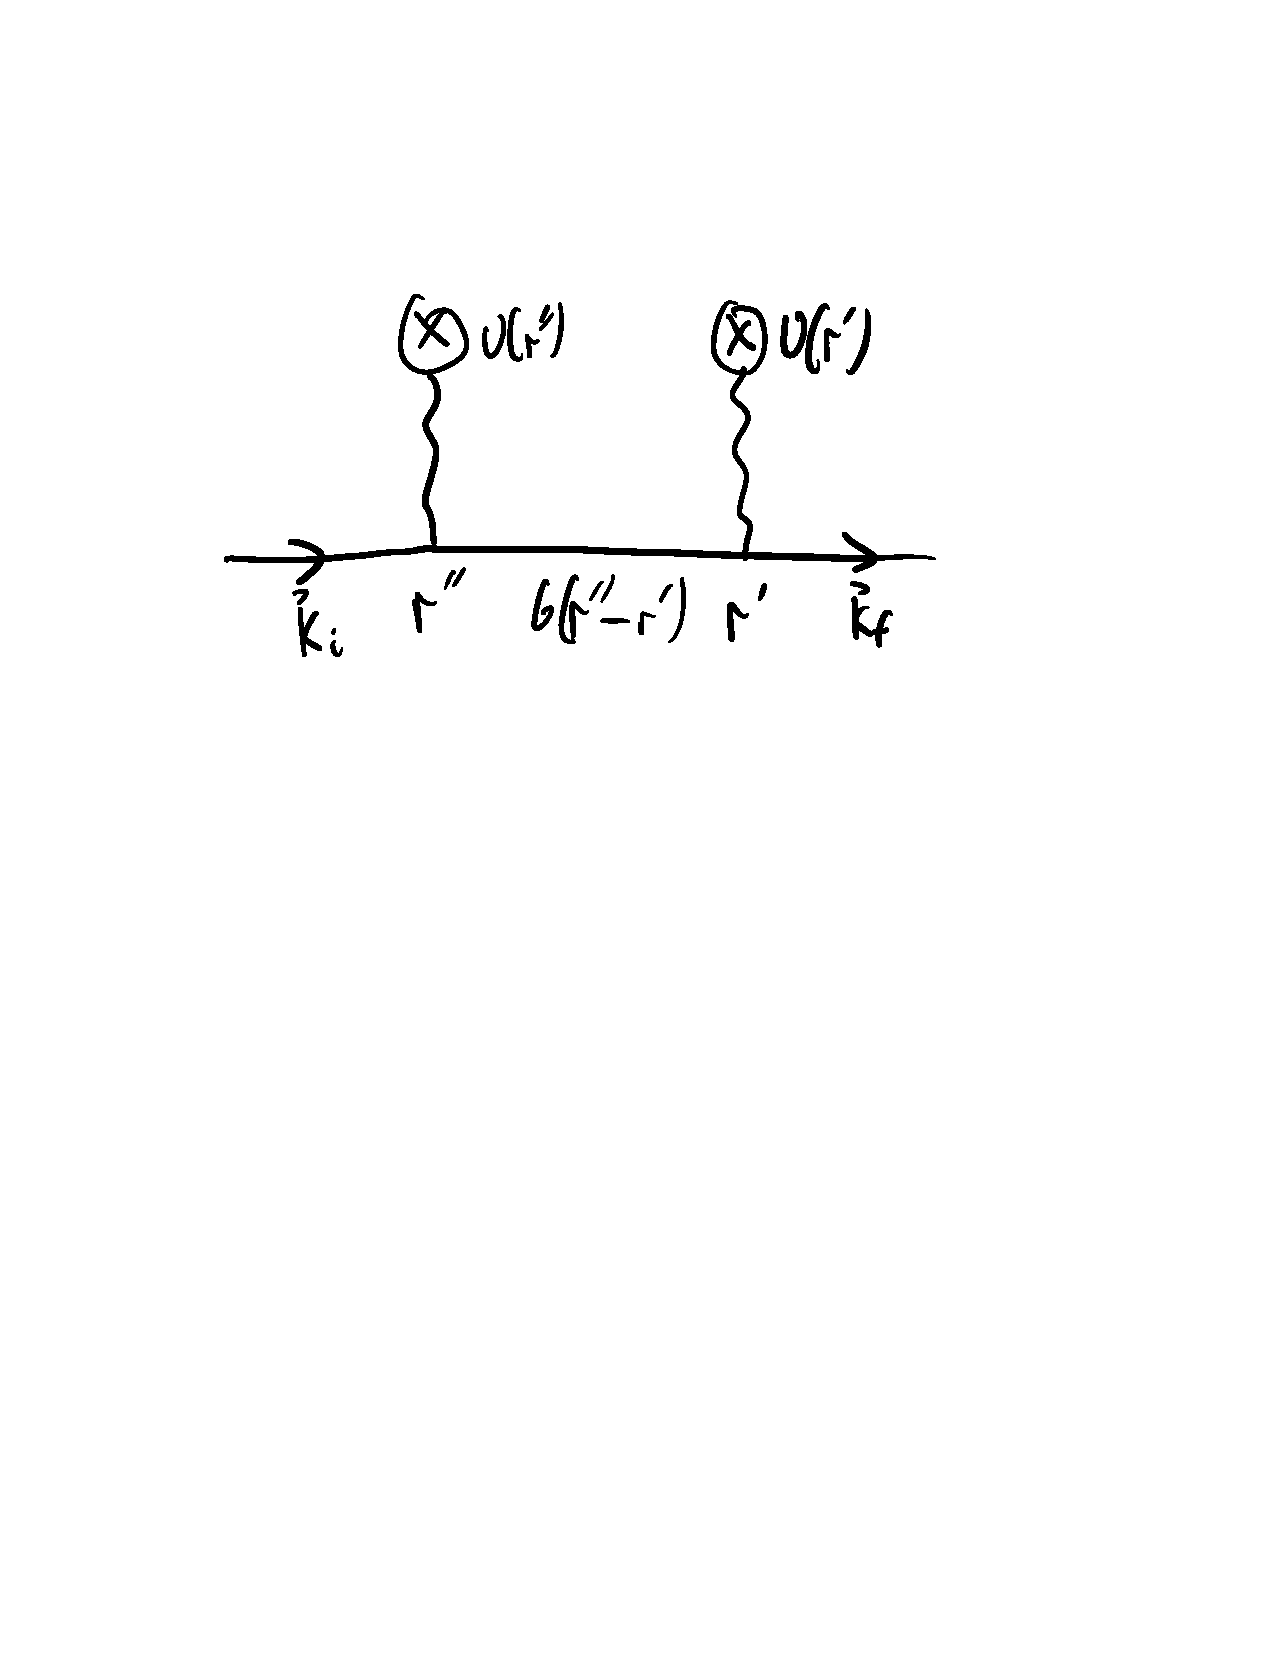
\includegraphics[scale=0.7]{Images/fig-feynmanscatter.pdf}
    \caption{Feynman diagram visualization for perturbation theory analysis of scattering.}
    \label{fig-feynmanscatter}
\end{figure}

These formulas were already known before 1947. But, Feynman wanted to visualize things in a way that would allow him to immediately write down the perturbation theory. We have an initial state $\ket{\psi_{in}} \cong e^{i\v{k}_i \cdot \v{r}}$ a final state $\bra{\psi_{out}} \cong e^{-i\v{k}_f \cdot \v{r}}$. The vertices are $U(r)$, the Propogator is $G(r' - r'')$. The way he visualized what was happening in PT was we have an initial momentum, then it starts to interact at $r = r''$, after interacting, it propogates with $G(r' - r'')$, then interacts again at $r = r'$, and then leaves as the final state. There is nothing new yet at this point, just a visualization of something we know. One can generalize this structure to quantum field theory.

One can discuss exactly the same Feynman diagram, but the interaction with a photon (or phonon, magnon etc. in CM physics) which represents the Compton effect:

\begin{figure}[htbp]
    \centering
    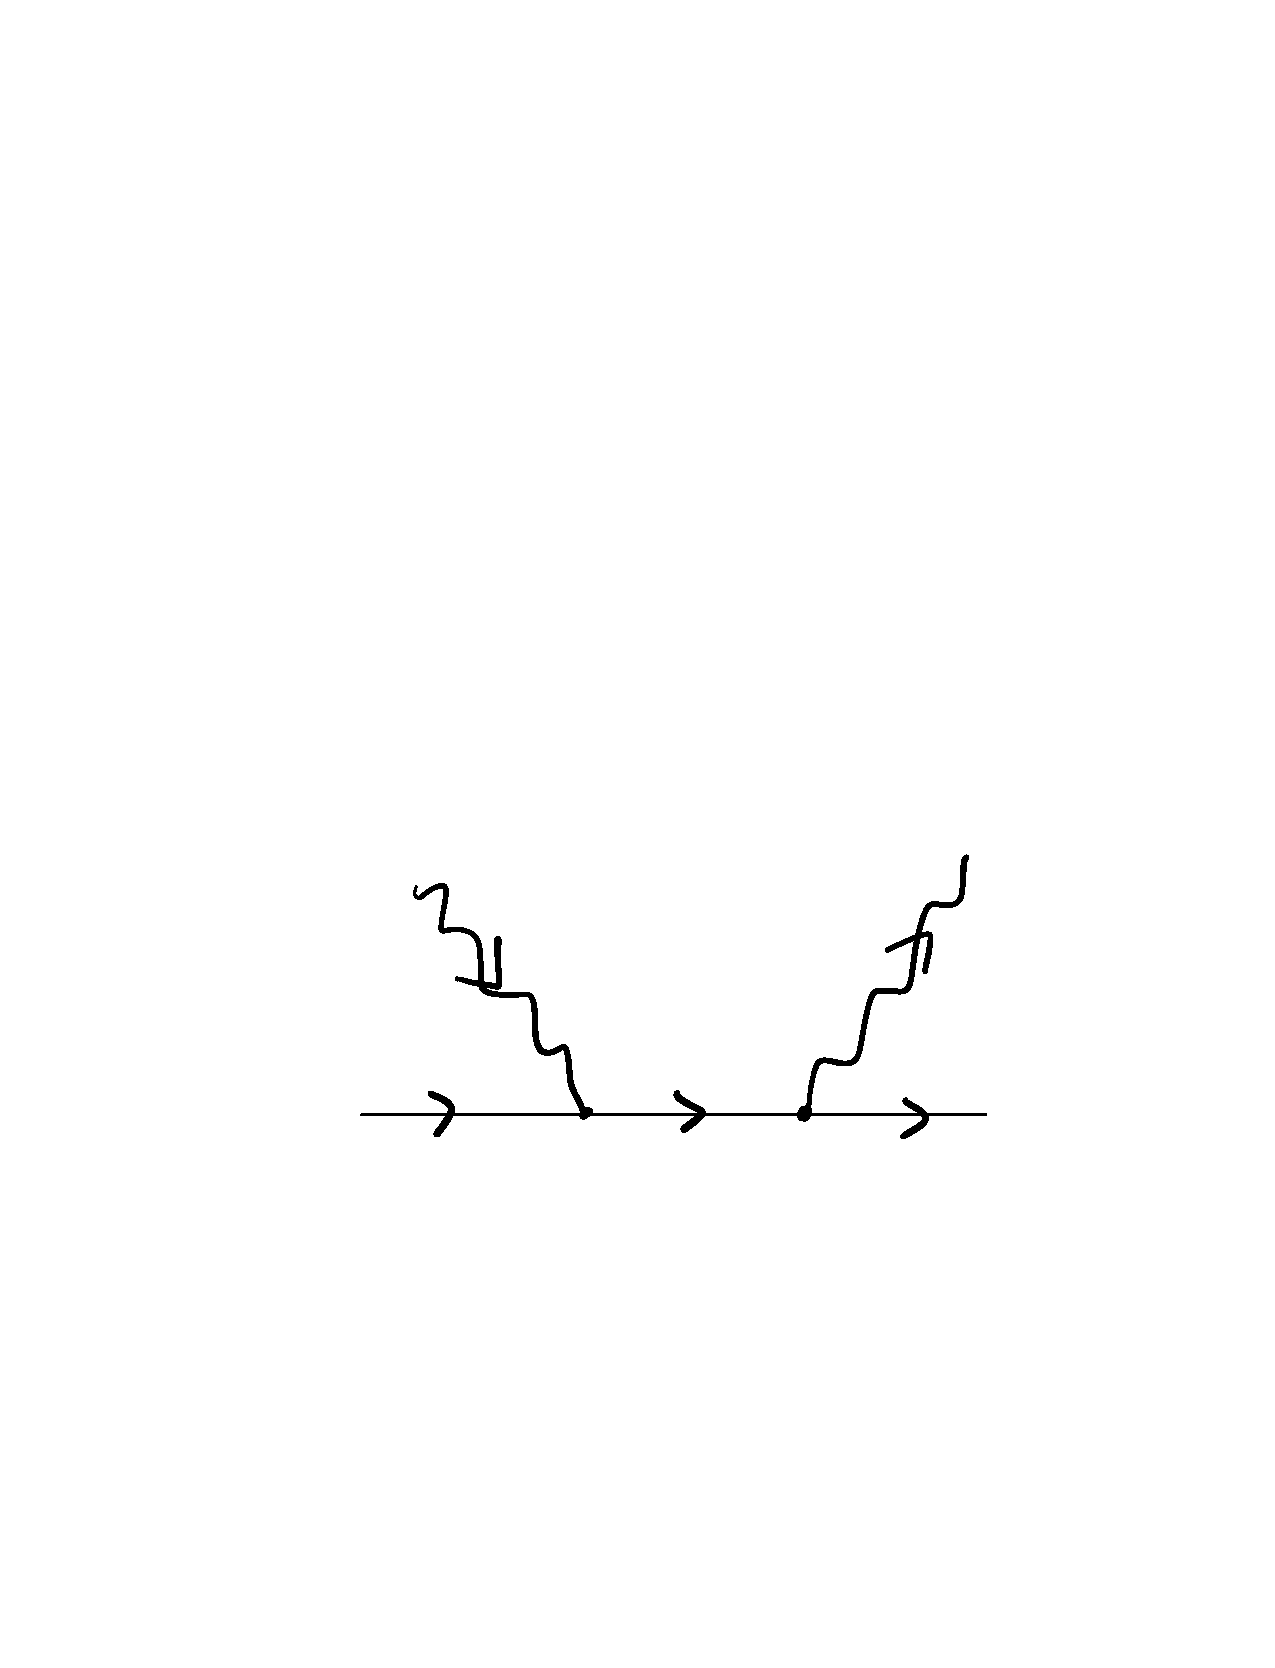
\includegraphics[scale=0.8]{Images/fig-feynmancompton.pdf}
    
    \caption{Feynman diagram for Compton scattering.}
    \label{fig-feynmancompton}
\end{figure}

\subsection{Justifying PT}
We unfortunately don't have time to discuss path integrals in this course - let's instead discuss the perturbation theory. In order for PT to be justified, we require:
\begin{equation}
    \abs{\psi^{(0)}} \gg \abs{\psi^{(1)}} \gg \abs{\psi^{(2)}} \gg \ldots
\end{equation}
Our condition is:
\begin{equation}
    \abs{\psi^{(0)}(r)} \gg \frac{2m}{4\pi \hbar^2}\int \frac{V(r')}{\abs{\v{r} - \v{r}'}}e^{ik\abs{\v{r} - \v{r}'}}\psi(r')d^3r'
\end{equation}
therefore:
\begin{equation}
    1 \gg \frac{m}{2\pi \hbar^2}\int \frac{V(r')}{r'}e^{ikr'}e^{-i\v{k}_i \cdot \v{r}'}d^3r'
\end{equation}
So for any potential, if this condition is satisfied we can use PT, if it is not we cannot.

\subsubsection{Low-Energy Regime}
We consider $ka \ll 1$, i.e. comparing the wavelength $\lambda$ with the length scale of the system. In this case, we can immediately due to the integration as the potential has a typical scale for which we can trivially carry out the integral. The exponentials are order 1, so we require:
\begin{equation}
    \frac{m}{2\pi \hbar^2} \abs{\int V(r') \frac{1}{r'}d^3r'} \ll 1
\end{equation}
Previously, we said that the amplitude $\abs{f} \ll a$; this is basically the same condition we had before. Before we just stated it without proof, now we see where it comes from.

\subsubsection{High-Energy Regime}
We consider $ka \gg q$. In this case we have to consider the integration over all angles. We consider:
\begin{equation}
    \int \sin\theta d\theta d\phi e^{-i\v{k}_i \cdot \v{r}'}r'^2 dr
\end{equation}
restricting our view to the angular part:
\begin{equation}
    \int \sin\theta d\theta d\phi e^{-i\v{k}_i \cdot \v{r}'} = \frac{2\pi}{\abs{\v{k}}\abs{\v{r}'}} \left(e^{ikr'} - e^{-ikr'}\right)
\end{equation}
Now multiplying by $\frac{V(r')}{r'}e^{ikr'}$:
\begin{equation}
    1 \gg \frac{m}{2\pi\hbar^2}\frac{2\pi}{k}\abs{\int \frac{V(r')}{r'^2}r'^2\left(e^{i2kr'} - 1\right)dr'}
\end{equation}
the only notable region of contribution is when $r' \gg k^{-1}$ (else $e^{i2kr'} - 1 \approx  1- 1 = 0$). So then the condition is:
\begin{equation}
    1 \gg \frac{m}{\hbar^2 k}\int_{r' \gg k^{-1}} V(r')dr'
\end{equation}

\subsection{Implications of Constraints}
Let's consider the trivial potential $V = -V_0, r \leq a$. For low energy ($ka \ll 1$), we have:
\begin{equation}
    \frac{mV_0}{2\pi \hbar^2} \int_0^a \frac{4\pi r^2}{r}dr = \frac{2m V_0}{\hbar^2}\frac{a^2}{2} \ll 1
\end{equation}
For high energy $ka \gg 1$, we have:
\begin{equation}
    \frac{m}{\hbar^2 k}\int V(r')dr' \ll 1 \implies \frac{mV_0 a}{\hbar^2 k} \ll 1 \implies \frac{mV_0 a^2}{\hbar^2} \ll ka
\end{equation}
What is the meaning of this condition? for any potential, so long as the energy is sufficiently large, my PT is justified. This is why PT is extremely useful for high-energy; no matter how high the potential is, the energy could be larger... so for large enough energies it is always justified.

Now, let's look at the Yukawa potential:
\begin{equation}
    V = \beta \frac{e^{-\mu r}}{r}
\end{equation}
For low energy, we have:
\begin{equation}
    \frac{m\beta}{2\pi \hbar^2}\int_0^{\infty}\frac{e^{-\mu r}}{r}\frac{1}{r}4\pi r^2 dr = \frac{m2}{\hbar^2}\frac{\beta}{\mu} \ll 1
\end{equation}
For the case of a Coloumb potential, $\beta = Ze^2$ and $\mu = \frac{\hbar^2}{me^2}$ and we see that the condition is never satisfied. We always have bound states. It is useless to consider PT for an atomic system. 

For high energy:
\begin{equation}
    1 \gg \frac{m}{\hbar^2 k}\int_{r' \gg k^{-1}}^\infty V(r')dr' = \frac{m\beta}{\hbar^2 k}\int_{r' \gg k^{-1}}^\infty \frac{e^{-\mu r'}dr'}{r'}
\end{equation}
This is formally divergent at the origin, but we have our cutoff at the lower bound, so $\int_{r \gg k^{-1}} \frac{dr}{r} \sim \ln \frac{\mu}{k}$. In any case this is of order one. So we study the constant out front:
\begin{equation}
    \frac{m\beta}{\hbar^2 k} = \frac{m\beta}{\hbar p_{ext}} = \frac{me^2}{\hbar p_{ext}} = \frac{me^2c}{\hbar c p_{ext}} = \frac{\beta c}{v_{ext} \hbar c} = \frac{\alpha c}{v_{ext}} \ll 1
\end{equation}
and so:
\begin{equation}
    \alpha \ll \frac{v_{ext}}{c}
\end{equation}
but since $\frac{v_{int}}{c} = \alpha$, we have:
\begin{equation}
    v_{int} \ll v_{ext}
\end{equation}

Conclusion: PT is useless if we want to probe structure - we develop tools for this next day. But at high energies everything works out.